%%%%%%%%%%%%%%%%%%%%%%%%%%%%%%%%%%%%%%%%%%%%%%%%%%%%%%%%%%
%%%%%%%%%%%%%%%%%% M A K R O S %%%%%%%%%%%%%%%%%%%%%%%%%%%
%%%%%%%%%%%%%%%%%%%%%%%%%%%%%%%%%%%%%%%%%%%%%%%%%%%%%%%%%%

%%%%%%%%%%%%%%%%%%%%%%%% g e n e r e l l e   M a k r o s %%%%%%%%%%%%%%%%%%%%%%%

%% 2019-07-26
%% phi@freimann.eu
%% Makros for BBW-Tex Documents


%%%%%%%%%%%%%%%%%% I N C L U D E S   &   I N D E X  %%%%%
\graphicspath{{../img/}}
\graphicspath{{./img/}}

\newcommand\bbwGraphicRaise[3]{\raisebox{#1}{\includegraphics[width=#2]{#3}}}%%
\newcommand\bbwGraphic[2]{\bbwGraphicRaise{-5mm}{#1}{#2}}%%
\newcommand\bbwCenterGraphicRaise[3]{\begin{center}\bbwGraphicRaise{#1}{#2}{#3}\end{center}}
\newcommand\bbwCenterGraphic[2]{\bbwCenterGraphicRaise{-5mm}{#1}{#2}}%%

%% Welche Zielgruppe soll ausgedruckt werden?
%% Typischerweise entweder TALS oder GESO (nicht beide). TRAINER ist optional für
%% die Trainer Version.
\newif\ifisTALS
\newif\ifisGESO
\newif\ifisTRAINER

\include{zielgruppe}

%% All in one Skript
\newif\ifisALLINONE
\isALLINONEfalse

%%%%%%%%% TRAINER Version vs. Schülerversion %%%%%%%%%%%%%

\newcommand\TRAINER[1]{%%
{%%
\ifisTRAINER{\color{BlueGreen}{#1}}%%
\fi%%
}}%%  

\newcommand\TALS[1]{%
{%%
\ifisTALS {#1}%%
\fi%%
}}%

\newcommand\GESO[1]{%
{%%
\ifisGESO {#1}%%
\fi%%
}}%    

\newcommand{\noTRAINER}[1]{{\ifisTRAINER{}\else{#1}\fi}{}}%%

%%\makeatletter
%% Je nach Umgebung "environment" wird das mmPapier breiter oder
%% schmaler
%% bei itemize sollen 16.4 und bei definiton-Boxen 16.8 mm genommen
%% werden.

\def\itemizeNAME{itemize}
\def\tcbNAME{tcb@savebox}
\newcommand{\TNT}[2]{\noTRAINER{

\ifx\@currenvir\itemizeNAME{}%% innerhlab von \begin{itemize} und \end{itzmize}
\renewcommand{\mmPapier}[1]{\mmPapierZwei{#1}{16.4}}%%
\fi%%
\ifx\@currenvir\tcbNAME{}%%  in rezepten, beipsielen, definitionen und gesetzen
\renewcommand{\mmPapier}[1]{\mmPapierZwei{#1}{16.8}}%%
\fi%%
\mmPapier{#1}%%
\renewcommand{\mmPapier}[1]{\mmPapierZwei{#1}{\defaultTextBreite}}%%
}\TRAINER{#2}%%
}%% END command TNT


%% Trainer "no" Dotfill
%% If no Trainer: Dotfill
\newcommand{\TNDF}[1]{\TRAINER{#1}\noTRAINER{\dotfill{}}}%%

\newcommand{\leserluft}{\vspace{2mm}}

%% Notiz felder 
%% Anwendung:
%% \noteField{10}  
%%  --> Notizfeld mit 10 Leerzeilen
\newcounter{DFCounter}

\newcommand*{\noteField}[1]{%
\setcounter{DFCounter}{1}
\vspace{0.5in}%
\begin{tabular}{p{14cm}}%
\hline%
\vspace{0.2cm}
Notizen: \\%
\whiledo{\theDFCounter < #1}{%
\dotfill \\
\addtocounter{DFCounter}{1}%
}%
\end{tabular}%
}%

\newcommand*{\noteLines}[1]{%
\setcounter{DFCounter}{1}
\vspace{0.1cm}%
\begin{tabular}{p{14cm}}%
\whiledo{\theDFCounter < #1}{%
\dotfill \\
\addtocounter{DFCounter}{1}%
}%
\end{tabular}%
}%

%% Platz für Notizen, aber nur bei Schülernverison (\noTRAINER)
\newcommand{\platzFuerTNNotes}[1]{%
\ifisTRAINER{}\else{%%
Platz für Notizen:\newline%%
\noteLines{#1}%%
}\fi{}%
}%%

%% Vier Leerzeilen für Notizen
\newcommand*\dotfillpara{%
\begin{tabular}{p{11.5cm}}%
\hfill   \\
\dotfill \\
\dotfill \\
\dotfill \\
\dotfill
\end{tabular}%
}


%%Häuschenpapier
\definecolor{bbblue}{rgb}{0.9,0.97,0.45}
\newcommand{\mmPapierZwei}[2]{\begin{tikzpicture}
  \draw[step=4mm,bbblue,thin]
  (0, 0) grid ({#2}, {#1});
  \end{tikzpicture}}%%

%% Standardbreite für Arbeitsblätter und das Theorieheft
%% Wird in bbwPruefung.sty überschrieben, da dort schmaler
\def\defaultTextBreite{17.6}
\def\unitCMWhatElse{cm}%% wird als Breitenangabe für den nächsten command verwendet

%% Verwendung: \bbwCenterGraphic{\defaultTextBreite}{«img url»}
\def\defaultTextBreiteCM{\defaultTextBreite\unitCMWhatElse}
\newcommand{\mmPapier}[1]{\mmPapierZwei{#1}{\defaultTextBreite}}


%% Notizen Berechungen auf Prüfungsblättern
\newcommand{\platzFuerBerechnungen}[1]{\noTRAINER{

Notizen / Berechnungen:

\mmPapier{#1}}}%% end platzFuerBerechnungen



\newcommand{\platzFuerBerechnungenOhneText}[1]{\noTRAINER{

\mmPapier{#1}}}


%% Die Abkürzung z.\,B. von «Zum Beispiel» hat einen verkleinerten Abstand.
\newcommand*\zB{%
z.\,B.
}

%%
%% Auf der Titelseite steht entweder GESO oder TALS.
%% Dies wird gleich mit der Fußnote angegeben.
%% Dieses Kommando sollte im Kommando «\untertitel» eingesetzt werden.
%%
\newcommand*\ausrichtungAufTitelseite{%
\ifisTALS{TALS\noTRAINER{\footnote{TALS «Technik, Architektur und Life Sciences
(Laboranten)»: Ausrichtung technisches Profil}}}%%
\fi%%
\ifisGESO{GESO\noTRAINER{\footnote{GESO: Ausrichtung \textbf{Ge}sundheit und \textbf{So}ziales}}}%%
\fi}%%

%%%%%%%%%%%%%%%%%%%%%% B B W - M a t h e   F a r b c o d e s  %%%%%%%%%%%%%%%%%%%%%%%%%%%%%%555

\newcommand{\rezeptFarbe}{red}
\newcommand{\definitionFarbe}{yellow}
\newcommand{\gesetzFarbe}{green}
\newcommand{\beispielFarbe}{orange}
\newcommand{\bemerkungFarbe}{orange}

%% Falls gewünscht übersteuren
%  \definecolor{xyz}{HTML}{eeff66}
%  \renewcommand{\beispielFarbe}{xyz}
%


%% Theorem-Styles
\newcommand\theoremlayoutdefinition[4]{\newtcbtheorem[number within=section]{#1}{#2}%
   {theorem style=plain,enhanced,colframe=#3!20!white,colback=#3!20!white,
     coltitle=#3!60!black,fonttitle=\upshape\bfseries,
     %%fontupper=\itshape,
    %%drop fuzzy shadow=blue!50!black!50!white,
    terminator sign={:},
    borderline north={0.5mm}{0pt}{#3}, borderline south={0.5mm}{0pt}{#3}
   }{#4}}



%% Farben für rezept, definition und gesetz von Marthale übernommen.
%% Verwendung mit * unterbindet die Nummerierung \begin{gesetz*}{Blah}{xy} ...\end {gesetz*}
\theoremlayoutdefinition{rezept}{Rezept}{\rezeptFarbe}{R}
\theoremlayoutdefinition{definition}{Definition}{\definitionFarbe}{D}
\theoremlayoutdefinition{gesetz}{Gesetz}{\gesetzFarbe}{G}%% was green
\theoremlayoutdefinition{beispiel}{Beispiel}{\beispielFarbe}{B}
\theoremlayoutdefinition{bemerkung}{Bemerkung}{\bemerkungFarbe}{M}


%% AadB = Aufgaben aus dem Buch
%% 1. Parameter: Seitenzahl
%% 2. Parameter: Aufgabennummern.
%% bsp  \TALSAadB{38-39}{101a-101c, 102 und 103}



\newcommand*{\maturaAufgaben}[1]{\begin{mdframed}[backgroundcolor=purple!10]{#1}\end{mdframed}}

\definecolor{shadecolor}{RGB}{180,180,250}
\newcommand*{\aufgabenfarbe}[1]{\begin{snugshade*}{#1}\end{snugshade*}}

\newcommand*{\aadB}{Aufgaben aus dem Buch}

\newcommand*{\TALSAadB}[2]{%%
{%%
\ifisTALS{\aufgabenfarbe{\noindent{\aadB \cite{frommenwiler17alg}: Seite {#1} Nr. {#2}}}}%%
\fi%%
}}%%

\newcommand*{\TALSGeomAadB}[2]{%%
{%%
\ifisTALS{\aufgabenfarbe{\noindent{\aadB \cite{frommenwiler18geom}: Seite {#1} Nr. {#2}}}}%%
\fi%%
}}%%

\newcommand*{\GESOAadB}[2]{%%
{%%
\ifisGESO{\aufgabenfarbe{\aadB \cite{marthaler21}: Seite {#1} Nr. {#2}}}%%
\fi%%
}}%%

\newcommand*{\theorieGESO}[2]{%%
{\ifisGESO{Theorie \cite{marthaler21}: Seite {#1} Kap. {#2}}%%
\fi%%
}}

\newcommand*{\theorieTALS}[2]{%%
{\ifisTALS{Theorie \cite{frommenwiler17alg}: Seite {#1} Kap. {#2}}%%
\fi%%
}}

\newcommand*{\theorieTALSGeom}[2]{%%
{\ifisTALS{Theorie \cite{frommenwiler18geom}: Seite {#1} Kap. {#2}}%%
\fi%%
}}

%%
%% Force a blank page, when \newpage does not work
%%
\def\blankpage{%
	\clearpage%
	\null%
	\clearpage}%%

\newcommand{\Lueckentext}[1]{\,\,\noTRAINER{\dotfill}\TRAINER{#1}}

\newcommand{\LoesungsRaum}[1]{\,\,\noTRAINER{\underline{\underline{\,\,\,\,\,\,\,\,\,\,\,\,\,\,\,\,\,\,\,\,\,\,\,\,\,\,}}}\TRAINER{#1}\,\,}

\newcommand{\LoesungsRaumKurz}[1]{\,\,\noTRAINER{\underline{\underline{\,\,\,\,\,\,\,\,\,\,\,}}}\TRAINER{#1}\,\,}

\newcommand{\LoesungsRaumLang}[1]{\,\,\noTRAINER{\underline{\underline{\,\,\,\,\,\,\,\,\,\,\,\,\,\,\,\,\,\,\,\,\,\,\,\,\,\,\,\,\,\,\,\,\,\,\,\,\,\,\,\,\,\,\,\,\,\,\,\,\,\,}}}\TRAINER{#1}\,\,}


%% TI nSpire
\def\tinspire{\texttt{TI-nSpire}}

%% TI 30 Pro Mathprint Button Images
\def\tiprobuttonbreite{10mm}
\def\nspirebuttonbreite{8.6mm}

%%\def\sec{\raisebox{-2mm}{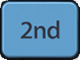
\includegraphics[width=\buttonbreite{}]{img/tiprobuttonimages/2nd.png}}}
\newcommand{\tiprobutton}[1]{\raisebox{-2mm}{\mbox{\,\includegraphics[width=\tiprobuttonbreite{}]{img/tiprobuttonimages/#1.png}\,}}}

\newcommand{\nspirebutton}[1]{\raisebox{-2mm}{\mbox{\,\includegraphics[width=\nspirebuttonbreite{}]{img/nspirebuttonimages/#1.png}\,}}}
